 %1-2 paragraph overview of science goals.  BAO, RSD, other applications.
 %SDT2015 as starting point.


%\begin{tcolorbox}[width=\textwidth,colback={mypink3},title={With true corners},outer arc=0mm,colupper=white]
%     Test
%     %%\includegraphics[scale=0.5]{frogimage.png}
%\end{tcolorbox}

%\begin{tcolorbox}[width=\textwidth,colback={coralpink},outer arc=0mm,colupper=white]
%     Test
%     %%\includegraphics[scale=0.5]{frogimage.png}
%\end{tcolorbox}

%\begin{textbox}[h]\section{SIDEBARS}
%Sidebar text goes here.
%\subsection{Sidebar Second-Level Heading}
%More text goes here.\subsubsection{Sidebar third-level heading}
%Text goes here.\end{textbox}


% Summary Points

% Future Issues

\begin{summary}
To mature the WFIRST GRS, our work has been organized along four main directions.
\begin{enumerate}
\item We developed, delivered to the project and updated the GRS requirements;
\item We generated new WFIRST specific light-cone simulations;
\item Using HST measurement, we started a new data analysis effort to improve our knowledge of the H$\alpha$ luminosity function, a critical element to plan the GRS;
\item We developed quick and agile analysis tools that will help us develop a pseudo-pipeline in the coming years.
\end{enumerate}
\end{summary}


 \subsection{Developing the GRS Requirements (D1)}

 \begin{summaryii}
   Over the last year, our main priority have been to support and guide the development of the WFIRST HLS spectroscopy and in particular to identify, articulate and validate the scientific requirements of the instrument, the data reduction software, and the survey. Responding to a calendar set by the Project Office, our SIT delivered three major updates to the WFIRST GRS requirements to the Project Office on July 1, 2016, December 1, 2016, and March 2, 2017. Each of these provide progressively sharper definitions of the  GRS requirements. We describe the main requirements and their science drivers below.
 \end{summaryii}

%This work was carried out by Wang, Eifler, Hirata, Ho, Kiessling, Krause, Merson, Padmanabhan, Pearson, Samushia, Benson, Capak, Dor\'e, Heitmann, Spergel, Teplitz, and Weinberg.

 \subsubsection{Science Requirements (Level 2a)} In this section we present the current level 2 science requirements as delivered to the Project Office. This section should be considered a snapshot as we will refine this requirements further in the coming years.
\label{sec:sr2a_grs}

 \paragraph{HLSS 1} The area to be surveyed shall be $\sim$1500 deg$^2$ (2000 deg$^2$ goal) after correcting for edge effects.  This area will be contiguous to the extent practical, and at least 90\% of the survey area must also be covered by the high latitude imaging survey.

 The survey area should be contiguous and large enough to reduce edge effects in
 the BAO/RSD measurements.  The $>90\%$ overlap with the HLIS enables joint
 analysis of 90\% of WL and GRS data, which maximizes the dark energy science
 from WFIRST.  Imaging also provides undispersed galaxy positions, improving
 redshift determination.  The statistical precision of the dark energy
 constraints is sensitive to the survey area as well as the survey depth; a trade
 study of depth versus area will need to be carried out to optimize both, in the
 context of Euclid and LSST. We also need to investigate the impact of dividing
 the area into two equal patches near the NEP and SEP respectively, to take
 advantage of potential ground-based telescope resources.  A survey of one or
 two large, contiguous areas has smaller edge effects and better window functions
 than a survey comprised of many smaller areas.

 We have carried out trade studies of the HLSS survey design. We note that it
 will be important to conducting these trade studies in the context of the joint
 science return of HLSS and HLIS that properly accounts for correlations among
 spectroscopic and imaging observables and accounts for their correlated
 systematics.  We are in the progress of implementing a corresponding forecasting
 effort.  Here, we have carried out a trade study of area versus depth for the
 HLSS only, starting from a baseline survey of 2227 deg$^2$ and a wavelength
 range of 1.05-1.85 microns. We consider two alternative scenarios, i.e. a survey
 twice as wide and shallower and a survey half as wide but correspondingly
 deeper.  The galaxy redshift distributions were computed using the WFIRST
 Exposure Time Calculator ETC v14. The H$\alpha$ forecasts are based on the average
 of the 3 models in \citet{Pozzetti:2016}, and the [O III] forecasts are based
 on the \citet{Mehta:2015} luminosity function.

 %The resulting redshift distributions are shown in Fig. 1.
 We extend the \CoLi framework \citep{Eifler:2014,Krause:2016jvl} to compute the constraining power of all scenarios on cosmic acceleration, closely following \citet{Wang2013}. We run 500,000 step
 MCMC simulated likelihood analysis in a 23 dimensional parameter space. We
 simultaneously vary 7 cosmological parameters and 16 ``nuisance'' parameters
 describing uncertainties due to the linear galaxy bias model, the non-linear
 smearing of the BAO feature, peculiar velocity dispersion, power spectrum shot
 noise, and redshift errors. We assume priors on cosmological parameters from the
 current state of the art experiments, i.e. the Planck mission, the Baryon
 Oscillation Spectroscopic Survey (BOSS), the Joint Lightcurve Analysis (JLA)
 supernovae, as described in \citet{Aubourg:2015}.

 The information gain is quantified using the standard Dark Energy Task Force FOM
 and an extended cosmology FOM, which measures the enclosed volume in the full
 7-dimensional cosmological parameter space, not just in the 2 dark energy
 parameters. We will refer to these FOMs as DE-FOM and Cosmo-FOM.  Compared to
 the baseline survey, we find a decreased DE-FOM of 32\% and a decreased
 Cosmo-FOM of 45\% for the shallow/large area survey. For the deep/small area
 survey we find an increased DE-FOM of 5\% and an increased Cosmo-FOM of 2\%.
 While our trade study validates the design of the baseline survey, we note that
 these findings are model and prior dependent and will carry out further studies
 varying the input parameters. In particular, the [OIII] galaxy number density
 will be updated pending inclusion of the results from the latest observational
 data from HST grism observations.

 %LS edited this paragraph. Added more detail.
 We also investigated whether the survey area needs to be contiguous. We
 constructed two identical sets of Gaussian simulations one set covering
 contiguous 2000 deg$^2$ and a second set consisting of two $1000$ deg$^2$
 disjoint fields. The BAO signal was then measured in the 2D power spectrum using the
 most recent techniques applied to the BOSS DR12 data. The BAO positions measured
 in disjoint fields were biased by 1\% on average compared to the contiguous
 field in both line-of-sight and transverse directions. This bias persists even
 after properly correcting for the window effects and is unlikely to be coming
 from the sample variance since our sets consisted of close to one thousand
 independent simulations. This bias could be a result of either bigger than the
 box-size modes or various edge effects. The window of the real data will be more
 involved than we considered in our test case and the biases may be larger. This
 investigation is ongoing but our preliminary results seem to support the
 conclusion that a contiguous area is preferable for the standard BAO analysis.

\paragraph{HLSS 2} The comoving density of galaxies with measured redshifts shall satisfy $n > 3\times10^{4}\ (h/\textrm{Mpc})^3$ at z=1.6.

 This is set by $nP_{0.2} \sim1$ at $z=1.6$, with 20\% margin. Requiring $nP_{0.2}
 \sim1$ implies $n> 3\times10^{-4}\ (h/\mathrm{Mpc})^{-3}$ at $z=1.3$, and $n >
 6.5\times �10^{-4} (h/\mathrm{Mpc})^{-3}$ at $z=1.8$. Given the Hirata
 forecast of H$\alpha$ ELG counts (Model 3 in \citet{Pozzetti:2016}, $nP_{0.2}\sim0.6$ at $z=1.8$,
 and $nP_{0.2}>2$ at $z=1.3$.  We cannot require a higher galaxy number density than
 what nature provides, given fixed observing time and area coverage. Here we have
 chosen a characteristic high redshift, $z=1.6$, at which it is impossible for a
 ground-based survey to obtain spectra for a large number of galaxies. There
 remain large uncertainties in the H$\alpha$ LF due to the limited availability of
 uniform data. It is likely that the actual number of H$\alpha$ ELGs is higher than
 assumed here; thus we have additional margins for this requirement. We have
 assumed a bias for H$\alpha$ ELGs of $b(z) = 1+0.5z$. The bias relation has been rescaled
 to agree with \citet{Geach2012} measurement of $b=2.4$ at $z=2.23$ for $f >
 5\times 10^{-17} \, \mathrm{ erg\,s^{-1}cm^{-2}}$.

 This is significantly deeper than the Euclid GRS survey, which ensures that the
 WFIRST GRS is deep enough for carrying out robust modeling of systematic effects
 for BAO/RSD, higher order statistics, and the combination of weak lensing and
 RSD as tests of GR. This number density requirement could in principle be met
 using either H$\alpha$ or [OIII] ELGs, depending on the survey strategy. There is no
 need to set a separate requirement for [OIII] ELGs; this depth ensures high
 number densities for both [OIII] and H$\alpha$ ELGs.

 Galaxy number density is a key input in the dark energy Figure-of-Merit. It
 is very sensitive to the H$\alpha$ LF, which still has large uncertainties but will
 become better determined as more data become available and more comprehensive
 analyses are done. The flow down of the galaxy number density requirement here
 to the minimum survey depth depends on the LF of ELGs.
 Co-I Teplitz is a key member of the WISP team. He is supervising a postdoc, Ivano Baronchelli, in deriving more precise LFs for H$\alpha$ and [OIII] ELGs using WISP data.

\paragraph{HLSS 3} The wavelength range of the HLSS will allow measurement of
H$\alpha$ emission line redshifts over the redshift range 1.1$<$z$<$1.9.

 The corresponding wavelength range is 1.38 $\mu$m to 1.9 $\mu$m.  This wavelength
 coverage also allows measurements of [OIII] emission line redshifts over the
 range $1.8 < z < 2.8$.  A wider wavelength range that allows H$\alpha$ emission line
 detection over a wider redshift range is desirable, as it increases the survey
 volume and therefore adds margin for meeting other baseline requirements.  It is
 also critical that the WFIRST GRS redshift range is complementary to that of
 Euclid, with its red cutoff at 1.85 $\mu$m, or $z < 1.8$.

 The key consideration is that a space mission should focus on what cannot be
 accomplished from the ground, and be complementary to other space missions in
 wavelength coverage. Ground-based GRS can reach $z\sim1$ without great difficulty,
 thus we should focus on $z>1$. Euclid GRS can only reach $z \sim2$; its shallow depth
 does not enable a high enough number density of observed [OIII] ELGs. WFIRST GRS
 is deep enough to observe both H$\alpha$ (656.3nm) and [OIII] (500nm) ELGs, with the
 number density of the latter sensitive to the survey depth (the deeper the
 survey the higher their number density).

 For the nominal wavelength range of 1-2 microns, WFIRST GRS covers $0.52 < z <
 2$ using H$\alpha$ ELGs, and $1 < z < 3$ using [OIII] ELGs. Thus the redshift range
 requirement is met including both types of ELGs.

 In addition to the trade studies in HLSS 1 we examine the impact of an extended
 wavelength range on the DE-FOM and the Cosmo-FOM. We follow the same methodology
 as detailed in the HLSS 1 description in extending the wavelength range from
 1.05-1.85 microns for the baseline model to 1.00-1.89 for the extended model.
 %The corresponding redshift distributions of the galaxy samples computed from the
 %ETC v1.14 are shown in Fig. 2.
 We find a decreased DE-FOM of 2\% and a decreased
 Cosmo-FOM of 11\% for the extended wavelength survey with respect to our
 baseline scenario. While the FoM trade study seems to favor a narrower redshift
 range, we emphasize that these findings are model and prior dependent and will
 conduct further studies varying the input parameters. The reduction in the
 telescope temperature to 260K will have a major impact on this trade study. In
 addition, the FoM comparison is quantitative but simplistic; it does not reflect
 how the various future surveys will complement each other. Euclid GRS covers the
 wavelength range of 0.92-1.85 microns using the same BAO/RSD tracers as WFIRST,
 thus there is unique scientific value in WFIRST having a wavelength cutoff
 longer than 1.85 microns.

\paragraph{HLSS 4} Redshift measurement errors $\sigma_z$ shall satisfy $\sigma_z < 0.001(1+z)$, excluding outliers, for galaxies smaller than $0.54''$ in radius. The fraction of outliers with $|z_\mathrm{obs}-
 z_\mathrm{true}|/(1+z_\mathrm{true})>0.003$ shall be less than 10\%.

 This is a requirement on the rms error of the redshift measurements, and not on
 every redshift measurement.

 We justify the requirement on the knowledge of the outlier fraction as follows.
 If you add a contaminant to the galaxy power spectrum with contamination
 fraction $\alpha$, then you leak in an amount of power from the "wrong" line
 with amplitude $\alpha^2$, but you dilute the power spectrum of the "real"
 signal by a factor of $(1-\alpha)^2$. For BAO the dilution is a minor issue (it
 reduces S/N), but for RSD it is a problem because it reduces the galaxy bias by
 $(1-\alpha)$ without changing the linear redshift-space distortion parameter
 $f\sigma_8$. So your inferred rate of growth of structure $f\sigma_8(z)$ is
 reduced by a factor of $1-\alpha$.  This leads to a stringent requirement on
 knowledge of $\alpha$ -- if it is 9.8\% but you think it is 10\% you have a
 0.2\% systematic error, which is a reasonable budget for this contribution.

 Larger size galaxies have larger redshift errors. To assess redshift accuracy,
 a realistic pixel level grism simulation covering at least 2 square degrees
 needs to be carried out and processed. The current data from the HST grism
 survey WISP finds that 90\% of galaxies that would be observed by WFIRST
 (H$\alpha$ flux $> 10^{-16} \mathrm{erg/s/cm}^2$, $0.55 < z < 1.85$) have a
 size less than $0.54''$ (semi-major axis continuum size). Since the maximum
 redshift of the WISP sample is $\sim1.6$, WFIRST H$\alpha$ ELGs will likely
 have smaller sizes on average, see Figure \ref{fig:size_zbin}.

 The [OIII] ELGs are more compact, so this requirement is also sufficient for
 the redshift precision for [OIII] ELGs.

\begin{figure}
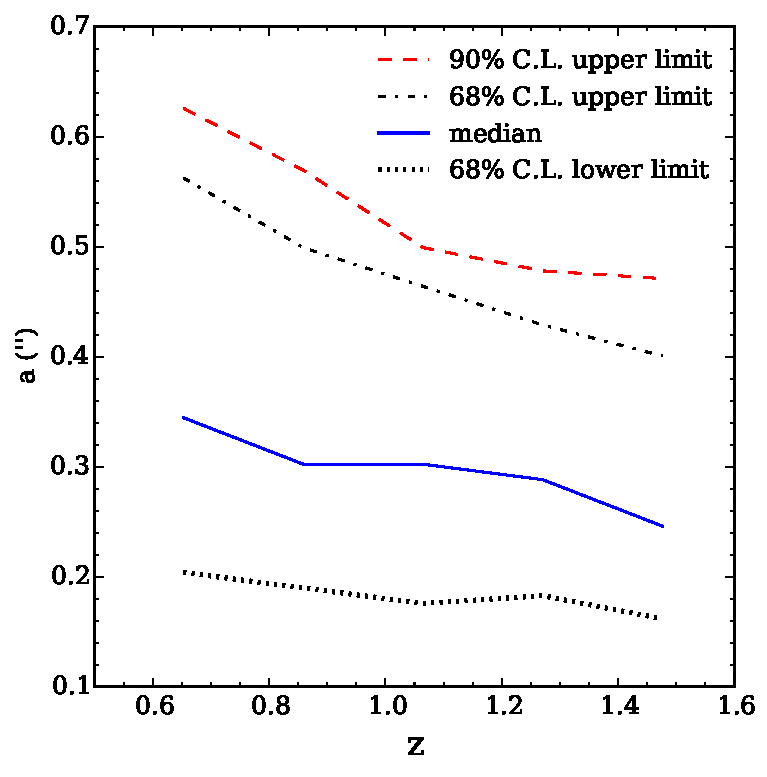
\includegraphics[width = 3.5in]{Plots/size_zbin.pdf}
\label{fig:size_zbin}
\caption{The 90\% upper limit of the semi-major axis
continuum size of H$\alpha$ galaxies with H$\alpha$ line flux $>10^{-16}
\mathrm{erg/s/cm}^2$, $0.55 < z < 1.85$), based on 1773 galaxies from WISP (WISP
team, private communication).} \end{figure}

\paragraph{HLSS 5} Relative position measurement uncertainties shall be less than $3.4''$ over the entire survey area.

 We need to measure galaxy positions to better than $\sim0.1 \mathrm{Mpc}/h$ (which corresponds to $3.4''$, assuming that 105 $\mathrm{Mpc/h}$ subtends 1 degree), in order to measure galaxy clustering accurately. This should be met easily if HLIS 26 is met, which makes systematic errors in the astrometry negligible. Given the pixel scale of $0.11''$, this requirement is automatically met within each field, and is tied to the precision of astrometry across different fields.

\paragraph{HLSS 6} The survey completeness shall be 50\% (TBC), and the redshift purity
 shall be 90\% (i.e., the outlier fraction is less than 10\%). Completeness is
 defined as the fraction of H$\alpha$ ELGs with measured redshifts flagged as reliable, and purity is defined as the fraction of measured redshifts flagged as reliable that are actually within 2$\sigma$ of the true redshifts.

 A requirement on completeness and purity is needed to translate the H$\alpha$ ELG
 number counts predicted by the H$\alpha$ LF to the galaxy number density that can be used to measure BAO/RSD by WFIRST GRS.  The completeness of 50\% and redshift
 purity of 90\% are put in as crude estimates based on extrapolations from
 Euclid.  Since WFIRST has a higher spatial and spectral resolution compared to
 Euclid, and more rolls (4 versus 3) per field, we expect a higher completeness
 and purity for WFIRST.  The actual requirements will need to be validated by
 grism simulations, since these are determined by what are feasible given the
 instrumentation and the true universe.  The requirement on the knowledge on the
 contamination fraction is set by HLSS 4.


 \subsubsection{Implementation Requirements (Level 2b)} In this section, we present the implementation requirements as delivered to the Project Office.

\paragraph{HLSS 7} The observatory shall provide a slitless spectroscopy mode, with a spectral dispersion no larger than 10.85 $\AA$/pix.

 Gratings tend to give constant dispersion in linear space, rather than R-space.
 The above dispersion would give point-source spectral resolution
 $R=\lambda/\Delta\lambda$ in the
 range $550 <R < 800$, for a 2-pixel resolution element.

 The grism resolution requirement is set by requiring the redshift precision to
 be 0.1\% (set by BAO/RSD science), thus is not sensitive to which ELGs (H$\alpha$
 vs [OIII]) we use as tracers. Going to lower spectral resolution would degrade
 the redshift precision and put BAO/RSD science goals at risk. The number density
 of [OIII] ELGs may be significantly higher than previously assumed; this gives
 some margin in the spectral resolution requirement due to the smaller sizes and
 less line blending of [OIII] ELGs.

 Given the margin from a likely higher [OIII] ELG number density than previously
 assumed, we have removed the requirement on resolving H$\alpha$ and NII for all
 galaxies of radius $0.3''$, and 90\% of galaxies of radius $0.54''$, which would drive
 the grism resolution higher. The blending of H$\alpha$ (6563$\AA$) and NII (6584$\AA$) leads to
 a metallicity-dependent shift in line centroid for larger sources
 this would lead to a systematic bias in the measured redshifts, which can
 propagate into the BAO/RSD measurements. Having a higher grism resolution would
 alleviate this problem, at the cost of a reduction in survey depth, and more
 overlapping of spectra for galaxies. This is a trade study that we will carry out
 as the required grism simulations become available.

 \paragraph{HLSS 8} Spectra shall achieve $S/N \geq 5$ for $r_\mathrm{eff} = 300
 \mathrm{mas}$ for an emission line flux $~ 1.0\times10^{-16}\ \mathrm{erg/cm}^2\mathrm{/s}$, from a source at 1.8 $\mu$m.

 This sensitivity is sufficient to meet the comoving space density requirement
 HLSS 2 with some margin given best estimates of the H$\alpha$ luminosity function
 \citep{Pozzetti:2016} at these redshifts. The use of a $\mathrm{S/N} \geq 5$ threshold for an arbitrary spectrum pre-spectral-decontamination gives margin for detection of sources whose spectra overlap others, or for loss of some exposures to cosmic ray hits or other artifacts, as $\mathrm{S/N} \geq 5$ post-decontamination is expected to be
 sufficient for meeting the redshift accuracy requirement HLSS 4, and the
 post-decontamination S/N should be significantly higher than the
 pre-decontamination S/N for a given spectrum. Current calculations of
 observatory performance indicate that the sensitivity specified here is achieved
 in a total exposure time of  $\sim1200$ seconds per field.

 The median continuum size (semi-major axis) of H$\alpha$ ELGs is $0.3''$ (see Figure \ref{fig:size_zbin}).
 This sensitivity requirement is phrased in parallel with the sensitivity requirement
 of the WL survey. This depth is a factor of two to three deeper than the Euclid
 GRS. The depth is sufficient to give the required galaxy number density in HLSS 2.

\paragraph{HLSS 9} The uncertainty of the wavelength measurement $\lambda$ shall satisfy $\Delta\lambda/\lambda \leq 0.001$.

 Although this is redundant since it is essentially the same as HLSS 4, it is
 necessary to keep it since it flows HLSS 4 into a dataset requirement.

\paragraph{HLSS 10} The spectroscopic bandpass shall satify $\lambda_\mathrm{max} \geq 1.9\ \mathrm{\mu m}$, and $\lambda_\mathrm{max}/\lambda_\mathrm{min} < 1.82$.

 We need $\lambda_\mathrm{max} > 1.9\ \mathrm{ \mu m}$ for redshift reach, in order to be complementary to Euclid and ground-based surveys.  Furthermore, we need $\lambda_\mathrm{max}/\lambda_\mathrm{min} < 1.82$ for line identification using multiple lines: to ensure that we cannot have [OII] (373nm) falling off the blue end of our coverage while H$\alpha$ (656.28nm) falls off the red end. We have
 assumed that the actual bandpass extends 1.5\% from either end, since it is
 problematic to use emission lines that fall within 1.5\% of the bandpass edges.

\paragraph{HLSS 11} 50\% of the energy (excluding diffraction spikes and non-1st order light) shall be enclosed in a circle of radius $<0.21^{\prime\prime}$ over 95\% of the field.

 This limit of $0.21^{\prime\prime}$ is required by source separation in the input
 catalog for spectral extraction, and is enabled by the addition of the phase
 mask corrector, and leaves some margin on the wavefront error.

\paragraph{HLSS 12} The filter used to define the bandpass of the grism shall have cutoff transition widths $\sigma < 1\%$ (0.7\% goal) after including the effects of broadening
 by the range of incident ray angles at each position in the FoV, where $\sigma$ is
 defined by $\sigma= (\lambda(T=0.90)- \lambda(T=0.10))/\lambda(T=0.50)$. $T$ is the transmission of the
 grism bandpass.

 This is based on the grism guiding considerations; the assessment of grism
 guiding (and its positive outcome) assumed $\sigma < 1\%$.

 \subsubsection{Implementation (Operations Concept) Requirements} We present here the implementation requirements related to the operation concept. We note that Co-I Hirata is the co-lead for the WFIRST Operations Working Group. We did not update Requirements HLSS 13-15, but include them here for completeness.

\paragraph{HLSS 13} Exposures of each field shall be obtained at a minimum of 3 dispersion directions, with two being nearly opposed.

\paragraph{HLSS 14} The observatory shall be able to place the WFC at a commanded
 orientation with an accuracy of $0.64^{\prime\prime}$ ($3\sigma$) in pitch and yaw, and $87^{\prime\prime}$ ($3\sigma$) in
 roll (TBR these were arbitrary values that give a net $3\sigma$ position uncertainty
 of 10 pixels. For the HLSS, the primary driver is that the position uncertainty
 is small with respect to chip gaps, which gives larger uncertainties than
 specified above. The smaller values quoted here are consistent with efficient
 target acquisitions, which would flow down from an observing efficiency spec.)

\paragraph{HLSS 15} The observatory pointing jitter and drift shall not exceed 100 mas in the spectral direction on the WFC focal plane (goal of 60 mas) and 50 mas in the cross- dispersion direction (TBR).

\paragraph{HLSS 16} Imaging observations shall be obtained of the fields in the HLSS that reach JAB=24.0, HAB=23.5, and F184AB=23.1 for an $r_\mathrm{eff}=0.3^{\prime\prime}$
 source at 10$\sigma$ to achieve a reference image position, in 3 filters.

 Provided the HLSS covers area already observed in the HLIS, this
 requirement will be met automatically.  This requirement applies to any HLSS
 fields that are counted toward the minimum survey area requirement but are not
 covered by the HLIS.  Imaging in at least three filters is required to build a
 minimal spectral template for grism spectral decontamination.

\paragraph{HLSS 17} There shall be 40 observations of two deep fields, each 11 deg$^2$ in area, sufficient to characterize the completeness and purity of the overall galaxy redshift sample. The 40 observations repeat the HLSS observing sequence of 4 exposures 10 times, with each deep field observation having the same exposure time as a wide field observation of the HLSS. The dispersion directions of the 40 observations should be roughly evenly distributed between 0 and 360 degrees.

To calibrate the HLS GRS, we need a spectroscopic subsample, with the same selection criteria as that of the HLS GRS, containing more than 160,000 galaxies  that have a redshift purity $>99\%$. We need 160,000 galaxies to know the redshift purity to 1\% (which requires 10,000 objects, assuming noise of $1/\sqrt{2N}$ from Poisson statistics) in at least four categories (low z, high z, faint, luminous).

Based on the estimated galaxy number density of $>7273$ per deg$^2$ at the flux limit for the GRS, $10^{-16} \mathrm{erg} \, \mathrm{s}^{-1}\mathrm{cm}^{-2}$, we need a total area for the deep fields of 160,000/7273=22 deg$^2$.  These can be split into two subfields of 11 deg$^2$ each.  Smaller subfields prevent the testing of galaxy clustering statistics in each subfield. Each deep field should be part of the HLS footprint, so they are representative of the GRS as a whole.

 The visits to the deep field should consist of 10 sets of HLS-GRS-like visits,
 matching the integration time, dither pattern, and observational time-sequence
 of the HLS-GRS strategy, with each set of HLS-GRS-like visits covering the same
 areas of 22 deg$^2$. Assuming a completeness of 50\% and uncorrelated sets, the
 completeness after 10 sets of visits is (1-0.5)10=0.001, leading to a 99.9\%
 complete sample for calibrating the GRS. Since each set of observation consists
 of 4 roll angles, the total number of deep field observations is 40. The
 dispersion directions of the 40 visits should be roughly evenly distributed
 between 0 and 360 degrees, in order to map out possible sources of systematic
 errors due to inhomogeneity.

\paragraph{HLSS 18} The observing efficiency of the HLSS, defined as the total science exposure time divided by the total time allocated to the survey, shall be TBD\%.

 The total time includes slew, settle, target acquisition, and
 calibration observations that are specific to the HLSS, including the
 extra-depth observations of the deep fields described in HLSS 17.  This minimum
 observing efficiency, together with a 0.67 year total allocation of observing
 time, allows science exposures of 1600 deg$^2$ (TBC) with the exposure time
 indicated in the comment to HLSS 8; this provides a 7\% (TBC) margin over the
 1500 deg$^2$ requirement (HLSS 1) to allow for data that may be unusable because of instrumental artifacts, bright sky objects, etc. This is a high level
 requirement that will need to be revisited as the mission implementation details
 become more solid; it should be set such that the core science goals for the GRS
 are achieved without putting mission success at risk.

\subsubsection{Calibration Requirements} In this section, we present the calibration requirements as delivered to the Project Office.

\paragraph{HLSS 19} The relative spectrophotometric flux calibration shall be known to 2 percent relative accuracy (with the goal of 1\%), in order to understand the effective sensitivity limit for each redshift bin for each area surveyed.

 The requirement here is only on the {\it relative} spectrophotometry, which impacts the selection function of galaxies. Absolute line flux calibration will only change the overall number of objects and the dN/dz, but will not introduce
 density variations.  Large scale structure measurements require precise
 knowledge of the selection function of galaxies. Although the overall redshift
 distribution may be determined by averaging over the entire survey, fluctuations
 in the selection function can easily contaminate the underlying cosmological
 density fluctuations.

 The spectroscopic sample for the GRS is expected to be defined by a line flux
 limit of 10$^{-16}\,$erg$\,$s$^{-1}$cm$^{-2}$. Spatial errors in the spectrophotometric calibration
 will introduce artificial spatial fluctuations in the number density of
 galaxies, which could contaminate the cosmological signal.

 We start by setting a requirement on the spatial uniformity of the mean number
 density as a function of physical scale. We require that the non-cosmological
 fluctuations in the mean number density (or the selection function of the
 survey) be $< 1\%$ (sqrt variance) when averaged over spatial scales between 10
 Mpc/$h$ to 200 Mpc/$h$. At small scales, this is $\sim$ two orders of magnitude smaller
 than the cosmological signal, while at the $\sim$ BAO scale of 100 Mpc/$h$, this
 is $\sim$ one
 order of magnitude smaller than the cosmological signal.  These fluctuations
 equal the cosmological signal at $\sim400 \mathrm{Mpc}/h$.  These physical scales correspond
 to $\sim0.5$ degrees to 6 degrees at a redshift of 1.5.

 We convert the above requirement to a requirement on the spectrophotometric
 calibration accuracy, assuming the Model I luminosity function of \citet{Pozzetti:2016}. At the flux limit of WFIRST, this yields a requirement of 1\% relative spectrophotometric calibration, averaged over angular scales of 0.5 degrees to 6 degrees.

 This is a very stringent requirement. We have relaxed this requirement from 1\%
 to 2\% to add margin for mission success, assuming that we will achieve 1\%
 relative spectrophotometric flux calibration in post-processing by projecting
 out problematic modes in the analysis.

 We plan to make this requirement more precise, in the form of "The relative
 spectrophotometric flux shall be known to 2\% relative accuracy in TBD (probably
 the spectral resolution) wavelength bins with a goal of 1\% on scales larger
 than TBD (per pointing, 0.3 deg) and TBD\% on scales smaller than 0.3 deg.
 We are working on deriving and justifying these numbers.
 Co-I's Capak, Hirata, and Padmanabhan are members of the WFIRST Calibration Working Group, working on a detailed calibration strategy for WFIRST.


\paragraph{HLSS 20} The uncertainty in the wavelength calibration shall not introduce biases in the wavelength measurement by amounts greater than
 $\Delta\lambda/\lambda = 10^{-4}$ on any
 angular scales exceeding 0.064 degrees within a field, and
 $\Delta\lambda/\lambda = 2\times10^{-5}$ from
 field to field.

 Variations in the wavelength calibration within a field, and from field to field
 on large scales, wash out the clustering signal by de-correlating the projected
 component of the clustering signal on those angular scales.

 Within a field, the acceptable level of wavelength error is
 $\Delta\lambda/\lambda \sim 10^{-4}$, which
 is 10\% of the errors on individual redshift measurements (0.001), to avoid
 increasing the overall redshift error by a significant factor. The angular scale
 is set by the optimal smoothing scale for BAO reconstruction, $\sim 5 \,
 \mathrm{Mpc}/h$. At $z=3$, this subtends 0.064 degrees for a flat universe with
 $\Omega_\mathrm{m}=0.3$ and a cosmological constant.

 For field to field, the acceptable level of wavelength error is $2\times10^{-5}$, which comes from comparing two adjacent fields.  Since we expect $\sim 104$ galaxies per deg$^2$, we have $\sim 2810$ galaxies per FOV of 0.281 deg$^2$.  If the galaxies have a redshift error of $10^{-3}$ each, then one can measure systematic offsets between fields (statistically) at the $10^{-3}/\sqrt{2810}$ level, which is $1.9\times10^{-5}$. At that level the power from the systematics is sub-dominant to the power from the redshift error.

 \subsubsection{Requirements on Science Data Products:} In this section, we present the GRS requirements on science data products. We are in the process of studying HLSS 21-25. These depend on the structure and responsibilities of the SOCs and the SITs. Co-Is Teplitz and Capak have extensive experience in data processing for space missions, and have provided detailed comments on these requirements to the WFIRST Project Office.

\paragraph{HLSS 21} The raw data for each grism exposure shall be available through the
 archive, with each dataset including identifying information such as time of
 exposure, observatory pointing orientation, a unique dataset identifier, and any
 engineering information needed for subsequent processing. Each detector readout
 for a given exposure shall be included in the dataset.

\paragraph{HLSS 22} Calibrated data for each grism exposure shall be available through the archive. Each detector readout shall be calibrated at the appropriate level, and the individual calibrated readouts will be combined to produce a net spectral image. These datasets shall include information on the effective PSF as a
 function of position and incorporate any World Coordinate System information
 needed for subsequent stages of processing. As sources are not yet identified,
 association of a pixel with a source position and wavelength is not yet
 possible.

\paragraph{HLSS 23} Source catalogs of the same field derived from WFC imaging data shall be combined with observatory pointing information for each grism exposure to produce a segmentation map that associates each catalog source with a range of spectral image pixels. The spectral images of bright stars in each detector shall be used to refine the astrometric solution.  These segmentation maps shall be used to extract 1D spectra for each source, and to flag pixels that may contain flux from multiple sources. The extracted spectra shall include
 information on the effective exposure time for each pixel, effective PSF as a
 function of position, data quality flags, and any other information needed to
 interpret the data.

\paragraph{HLSS 24} Extracted spectra of each source from multiple roll angles shall be
 combined to produce a single net spectrum of each source. For sources that are
 spatially resolved, the result shall be provided as a data cube of position and
 wavelength. The spectra obtained at nearly opposing roll angles shall be used to
 account for possible offsets of the emitting region from the center of the
 broad-band image. The data from all roll angles shall be used, to the extent
 possible, to resolve ambiguities in the proper source to associate with pixels
 illuminated by overlapping spectra. These net spectra shall include information
 on the effective exposure time for each pixel, statistical and systematic
 uncertainties in the measured fluxes and wavelengths, effective PSF as a
 function of position, data quality flags, and any other information needed to
 interpret the data.

\paragraph{HLSS 25} The data processing system shall have the capability of inserting fake sources into the spectral image data and re-executing the generation of
 high-level science products. These tests are essential for verifying the proper
 operation of the tools that generate high level science products and for
 understanding the sensitivity of the survey and systematic effects that may be
 present in the survey sample.

\paragraph{HLSS 26} The data processing system shall provide sufficient knowledge of the 3D selection function so that the artificial correlations due to inaccuracies in the 3D selection function are less than 10\% of the statistical error bars on
 scales smaller than 2 degrees, and less than 20\% on larger angular scales.

 This requirement is only meaningful in terms of the contribution to the total
 error budget by the uncertainties in the 3D selection function. The BAO scale is
 less than 2 degrees in the redshift range for the HLSS.

 To convert the positions of observed galaxies in the large-scale structure
 into clustering measurements (correlation function, power spectrum, higher order
 statistics) we need to know how the "average" number density of objects (in the
 absence of clustering) changes in the observed volume. The mean number density
 will vary significantly both in redshift and with angular position due to
 effects of target selection, data reduction and observing conditions. Previous
 surveys were able to separate the selection function in two independent parts:
 the radial selection function and the angular selection function. It is likely
 that the WFIRST selection function will not be separable in this way, i.e.
 different parts of the sky will have different radial profiles. For now we will
 assume that this type of separation is possible. This assumption is reasonable
 for preliminary investigation since most effects are either mostly radial (e.g.
 target selection, data reduction) or angular (e.g. imaging quality, galactic
 extinction).

 The knowledge about 3D selection function is usually encoded into sets of random
 catalogues. When computing clustering statistics, the random catalogues remove
 the systematic effects of varying mean number density (due to target selection,
 data reduction or observing conditions). If the 3D selection function is not
 correct, the effects will not be completely removed and will generate spurious
 correlations that can bias the true cosmological signal. The angular mask of the
 WFIRST data will vary pixel to pixel on the infrared detector. The full
 description of the angular mask may turn out to be computationally intractable.
 For the core science goals we require the description of the mask to be correct
 with an angular resolution of approximately 3 arcmin. This corresponds to a
 spatial resolution of $3 \,h^{-1} \mathrm{Mpc}$ at $z=1.5$. This is driven by the fact that we
 need to be  able to resolve the BAO peak. In principle, our requirements on the
 knowledge of the 3D selection function are driven by the main requirement that
 the spurious correlations should be no more than TBD per cent of statistical
 errors between the scales of 10 and 150 h-­?1Mpc in clustering signals (either
 in correlation function multipoles or power-­?spectrum). For the galaxy sample
 expected from WFIRST, this corresponds to TBD per cent uncertainty in the
 knowledge of the radial distribution and the angular mask.

 To further quantify the effect of systematics offset in the angular mask on
 clustering measurements we have performed tests on mock catalogues representing
 BOSS CMASS sample. This is justified by the fact that the BAO and growth rate
 measurements from WFIRST GRS in redshift bins of $z\sim0.1$ are expected to be
 roughly equal to the CMASS constraints with $z\sim0.2$.

 The mock surveys are generated from N-body simulations, with a median redshift
 of 0.6, with galaxies of halo mass range about $7\times10^{13}\,M_\odot$. The mock
 surveys have proper BOSS 3D selection function (which we take as truth here).
 Now we distort the selection function in the following scenarios:


\begin{figure}
 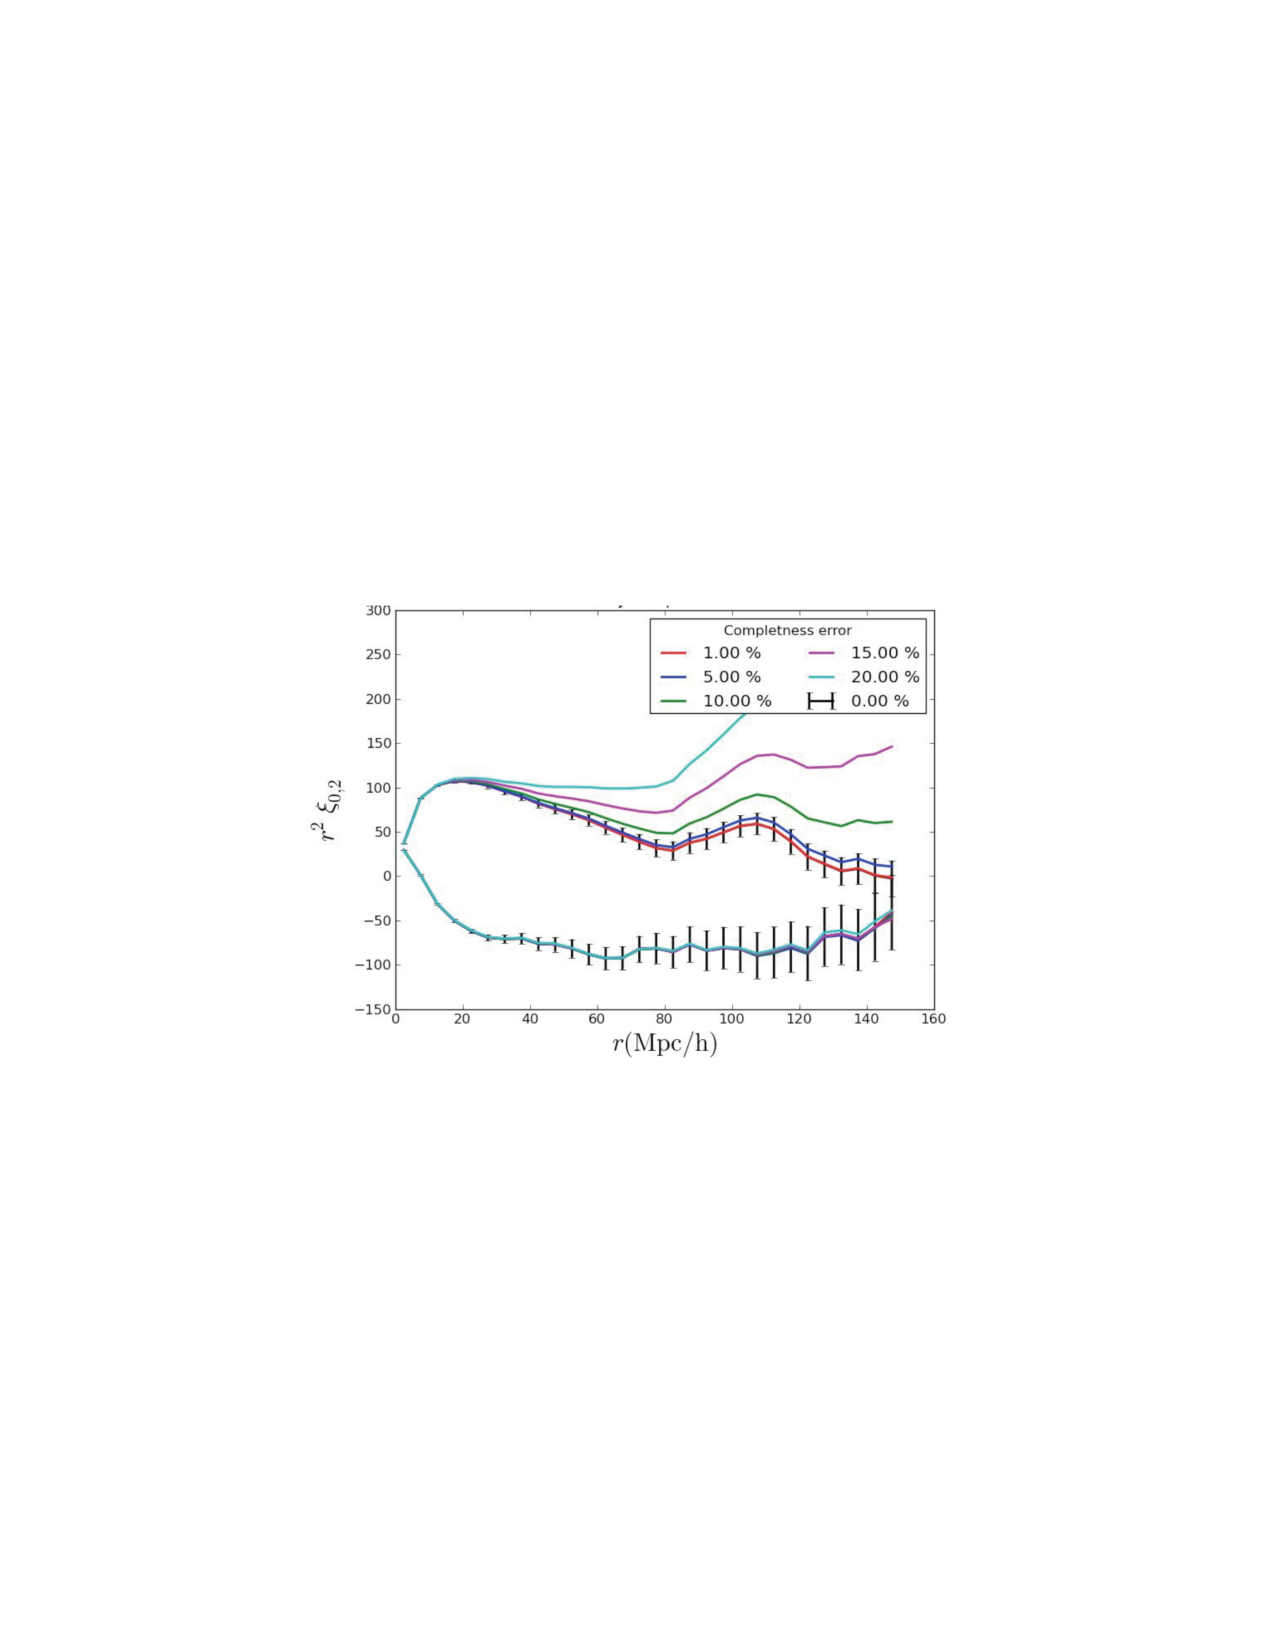
\includegraphics[width =0.75\textwidth]{Plots/GRS_req_1July2016_v3_P6fig.pdf}
 \label{fig:selection_function}
 \caption{The monopole (upper curves) and quadrupole (lower curves) of a single mock survey and how they respond to various completeness errors in the scenario described in scenario. We can see from the level of two point correlation function, even a 5\% error on the completeness can change the monopole   and quadrupole significantly that we expect RSD to be affected, while BAO is not significantly affected, as this mostly changes the amplitude of the correlation function.}
  \end{figure}

\begin{enumerate}
\item The survey region is divided into two equal area along RA and one area
 has true completeness whereas the other one has $1-x$ completeness where x is a
 given completeness error (as shown in the legend of Figure~\ref{fig:selection_function}).
 We show in Figure \ref{fig:selection_function} the resulting monopole and quadrupole with varying completeness error. This
 is an interesting limiting case as surveys can sometimes be affected by large
 scale systematics generated by either calibration of two parts of the sky, or
 due to large scale effects caused by the galactic foregrounds.
\item The true survey completeness is multiplied with a gaussian function. The
 gaussian function has mean 0 and variance as the denoted completeness error. We
 then fold both positive and negative side of the Gaussian to the negative side
 and hence allow the completeness to be only smaller than its true value. We vary
 the scale at which we change the 3D selection function, starting with 1 degree
 to 4 degrees (4 deg. is approximately the BAO scale at this redshift).
 \end{enumerate}
 %In particular, we will show the resulting monopole and quadrupole for 2 degrees and
 %4 degrees in Figure 3 and Figure 4 respectively. These are two interesting
 %limiting cases since they correspond to the extreme situation when the 3D
 %selection function are changed at scales most relevant to linear RSD modeling
 %and BAO analysis.

 From the preliminary analysis shown here, we expect that we will need to
 accurately model the 3D completeness function down to a few \% level.  At 5\%
 the effects can already be very detrimental to our large scale structure
 analyses using BAO and RSD. Scaling from these, we arrive at the requirement
 that artificial correlations due to inaccuracies in the 3D selection function
 are less than 10\% of the statistical error bars on scales smaller than 2
 degrees, and less than 20\% on larger angular scales.

 \subsubsection{Requirement on Cosmological Volume Simulations:} We now present a new category of requirements for a space mission. These are not needed
 for mission success (data acquisition by the spacecraft), but only for meeting the
 high level science requirements (level 1). We summarize these as follows:

 \begin{enumerate}
 \item a few accurate mocks with galaxies included using semi-analytical
 galaxy formation model, to verify and validate WFIRST GRS pipeline;
 \item $\sim 100$ mocks with high mass resolution of 109 solar masses, to inform theoretical modeling of the data;
 \item $\sim 10,000$ mocks with low resolution, to derive the covariance matrices for the WFIRST data.
 \end{enumerate}

 To quantify the requirement on cosmological volume simulations, we consider only
 the case for galaxy clustering science (which includes BAO and RSD) for now for
 simplicity. For WFIRST, simulations are required for the following three
 objectives:
\begin{enumerate}
\item establishing the basic correctness of the pipeline;
\item informing the theoretical modeling of small scale clustering as a function of
 tracer properties;
 \item calculating the covariance matrix for each GRS probe and
 across many probes.
 \end{enumerate}

 In order to establish the basic correctness of the WFIRST pipelines and
 predictions, sophisticated synthetic mock galaxy catalogs are essential.
 These catalogs, which must realistically emulate WFIRST both in sky area and
 depth, are typically constructed by running large gravity-only simulations and
 then ``painting'' realistic galaxies on top.  Populating a simulation with
 galaxies can be done in several ways: (i) empirically, using statistics such as
 the ``halo occupation distribution'', (ii) by placing the normal, baryonic matter
 in the simulation ab initio and explicitly solving the hydro-dynamical
 equations, or (iii) by using a semi-analytical galaxy formation model (SAM),
 whereby the astrophysical processes and formation histories of galaxies are
 described using physically motivated, parameterized equations. The advantage of
 SAMs over alternative methods is their ability to meet the demands from next
 generation cosmological surveys for large (suites of) galaxy mock catalogues
 that are both accurate and can be constructed rapidly. In contrast, full
 hydro-dynamical simulations are far too slow and empirical methods are limited
 by the availability of existing high redshift observations, which are necessary
 for the calibration of these methods. SAMs also require some observations for
 calibration but, once tuned to fit observations at low redshift, they are able
 to make predictions out to high redshift without the need for further
 observational input. Furthermore, empirical methods are often limited in that
 they are calibrated in one or two photometric bands, whilst SAMs are designed to
 model the star formation history of a galaxy and so have the ability to make
 predictions for a wide variety of multi-wavelength data simultaneously. This
 feature of SAMs is vital to ensure that we can examine cross-correlations
 between the spectroscopically-selected dataset for galaxy clustering analysis
 and the photometrically-selected dataset for weak lensing analysis. Besides
 testing the pipeline and making (limited) cosmological forecasts, these galaxy
 mock catalogs would also be a valuable resource for science working groups
 focusing on legacy science (e.g. galaxy evolution, active galactic nuclei). Note
 that,  compared to the large number of approximate mock catalogs necessary for
 covariance estimation, only very few accurate galaxy mocks are required to
 verify and validate the WFIRST pipeline.


 To inform the theoretical modeling of clustering especially at non-linear
 scales as a function of the tracer properties would require a significant number
 of simulations that have relatively realistic modeling of the tracer properties
 at the relevant redshift.  For WFIRST, we can take the current number density of
 emission line galaxies (for H$\alpha$ galaxies only) from our baseline
 calculation and used the \citet{Tinker2008} halo mass function, along with the
 \citet{Giocoli2008} subhalo mass functions to compute the total number of
 halos and subhalos above some mass threshold and then match that to the baseline
 GRS number densities. This maps back to approximately 10$^12$ solar masses from z=1 to z=2. Assuming that we need to have at least 100 particles to resolve halos at
 1012 solar masses, and another factor of 10 particles to resolve properties of
 the halo progenitors, we will need dark matter particle mass resolution of
 approximately 10$^9$ solar masses. The extra factor of 10 is due to the galaxy
 formation model that depends on the properties of the progenitors which is an
 approximation that may change as we understand the galaxy properties better and
 as more observations of the tracers arrive. We expect to require of order 100
 simulations to reduce the shot noise of the correlation function in order to
 compare the theoretical modeling to the simulated correlation function. These
 realistic mock surveys may also require the modeling of non-standard
 cosmological  models, such as extensions to non-zero total neutrino masses, or
 modified gravity models.

 Finally, we will need to calculate the covariance matrices of the main probes of
 clustering, namely BAO and RSD, and the cross-covariances among these probes
 (or across different methods as in recent BOSS analyses). We can approach the
 calculation of the covariance matrices through multiple avenues. One can
 generate (in principle) a large number of approximate mock surveys using
 relatively fast approximate methods (eg., PTHalos, QPM, FastPM, etc), and apply
 the relevant survey properties onto these mock surveys. The small scale modeling
 of the clustering may not be 100\% accurate, but is likely to be adequate for
 the linear RSD modeling and BAO analyses where medium to large scales are most
 important. The number of approximate simulations required can be on the order of
 O(10,000) depending on the number of parameters we will be estimating using
 these covariance matrices, but the time requirement of these approximate mocks
 is relatively modest. One can also envision using more theoretical approaches
 (such as \citet{OConnell:2015src,Padmanabhan2016,Friedrich:2015nga}, which only require a relatively modest number of realistic mock surveys which are required for (b).


\subsection{GRS Light-cone Simulations (D8 and D9)}
%--------------------------------------------------

 \begin{summaryii}
Light-cone cosmological simulations are a critical tool to design the GRS survey design, to develop and to validate analysis tools and theoretical predictions. We developed four complementary simulation approaches to tackle multiple questions relevant to the GRS:
\begin{enumerate}
  \item A lognormal simulation to generate quickly large cosmological volumes;
  \item A fast approach using simple galaxy-halo prescriptions to generate joint GRS and WL simulations;
  \item A realistic emission line galaxies modeling to study the confusion between H$\beta$ and [O III] emitters;
  \item A realistic semi-analytic galaxy evolution model to make robust H$\alpha$ mock catalogs.
 \end{enumerate}
 \end{summaryii}

 In order for WFIRST HLS to reach its  high level science requirements, we have
 proposed to ({\bf D9})  produce simulated light-cone observations to ({\bf D8})
 develop both the methods for modeling and interpretation of cosmological
 measurements from WFIRST.  Most of these data sets will be at the level of
 galaxy redshift and shape catalogs rather than the pixel-level imaging and
 spectroscopy simulations described above. They will incorporate varying degrees
 of complexity regarding galaxy bias, redshift evolution, survey geometry, and
 observational systematics such as incompleteness, shape measurement errors, and
 photometric redshift biases. Many of these artificial data sets will be made
 publicly available, and some will take the form of data challenges, where the
 underlying parameters are initially known only to the creators of the data set.
 Here we report on our first year simulation efforts  in a 4 prong approach,
 ranging from the largest volume to the highest resolution below:

\subsubsection{Lognormal Simulations}

 Samushia and his postdoc have produced a suit of few thousand fast
 ``enhanced log-normal simulations'' for the WFIRST GRS expected samples. While
 these simulations do  not correctly reproduce the small scale structure and
 higher order statistics of the field, they can be used for studying various
 large scale effects and implement light-cone effects. The simulations have so
 far been used to study the effect of splitting the WFIRST footprint into two
 non-contiguous areas. We plan to use these simulations in the future to study
 systematic effects in the measurements (e.g., window effect correction) and to
 validate the BAO/RSD proto-pipeline. These simulations are very well-suited for
 such tasks since their input two-point signal is known exactly.

 \subsubsection{Fast simulations with galaxy positions and shapes}

 Kiessling, and Huff are working with Postdoc Izard to develop a fast
 pipeline to provide galaxy mock catalogues with weak lensing. The goal of our
 initial project is to model effects of various systematics and determine their
 impact on galaxy clustering and weak lensing observables and their covariance
 matrices. The starting point for this project is  300 ICE-COLA fast simulations
 \cite{Tassev:2013pn,Izard:2015dja} generated by Izard during his PhD that
 provide the dark matter density field and halo catalogs (both in the light cone
 geometry). The former is used to compute maps of weak lensing distortions in
 the Born approximation using a technique developed by Izard (Izard et al, 2017;
 in prep). Galaxies are attached to halos using a new pipeline developed for
 this project. This pipeline takes the halo catalogues in the light cone
 geometry generated by the fast simulations and produces galaxy samples with
 broad band luminosities and weak lensing properties. The produced catalogs are
 all sky and span 0 $<$ z $<$ 1.4, with a minimum dark matter halo mass of
 $10^{12}  M_{sun}/h$.

 \subsubsection{Testing the effect of line confusions on BAO using N-body simulations}

  \begin{figure}
   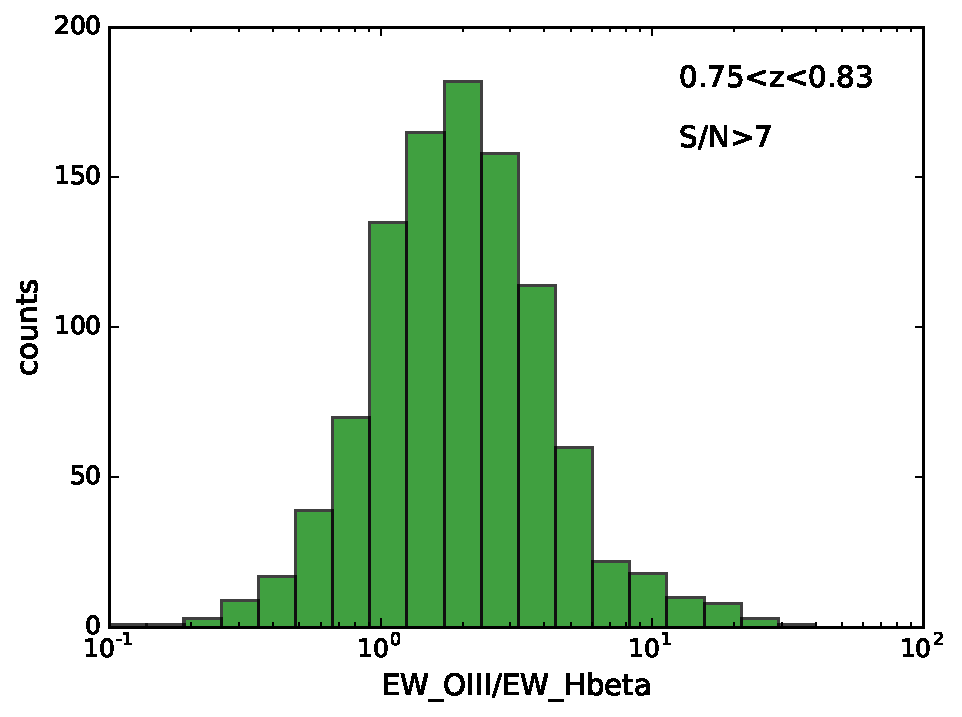
\includegraphics[width = 0.4\textwidth]{Plots/OIII-Hbeta.pdf}
  \label{fig:line-ratios}
   \caption{The line ratios between H$\beta$ and [O III] using the most up to date dataset from SDSS4-eBOSS, which currently has acquired over 10,000 emission line galaxies, but a significant fraction of them have H$\beta$ and/or [O III]. The plot shows $\approx$1000 galaxies from eBOSS sample that has both H$\beta$ and [O III], while each line is detected at least at 7-$\sigma$).}
  \end{figure}

 Ho and Massara concentrates on one particular goal in generating their simulations. Their goal is to investigate the effect of confusion between H$\beta$ and [O III] emitters, in particular in the high level science goal in BAO. In WFIRST,  the primary science targets for the redshift survey will be H$\alpha$ and [O III]. There is a special concern of H$\beta$ vs. [O III] confusion due to their proximity in wavelength (hence the inability of photo-z's to distinguish them reliably). This is particularly true given that an H$\beta$ emitter mis-identified as [O III] will have an inferred radial position different by 8900 km/s (or: 89 $h^{-1} Mpc$ * (1+z)/$\sqrt{\Omega_\Lambda + \Omega_m (1+z)^3}$, which in our range of redshifts is near the BAO scale). We will also get some [O II] emitters -- these might be useful directly for cosmology, or for disentangling other line emitters (see Pullen et al. 2014). Note that at WFIRST resolution 3726 and 2729 are a blend.

 A key challenge in the mocks will be making sure the populations of each line and the correlations among the different line strengths and with environment are sufficiently realistic for the tests we are doing. This has historically proven to be very difficult due to the heterogeneous nature of the observational constraints. Therefore, we have investigated the equivalent width ratio between H$\beta$ and [O III] using the most up to date dataset from SDSS4-eBOSS, which currently has acquired over 10,000 emission line galaxies, but a significant fraction of them have H$\beta$ and/or [O III]. This is so far the only statistical sample that can be used to look at the line ratios (see Figure~\ref{fig:line-ratios}). We also look at the conditional luminosity function between the two line luminosity and found them to be consistent with what was observed in DEEP2 (see Figure~\ref{fig:cond-lum}) with higher statistics. We now proceed to use these line ratios to create the emission line galaxy catalog.

 \begin{figure}
  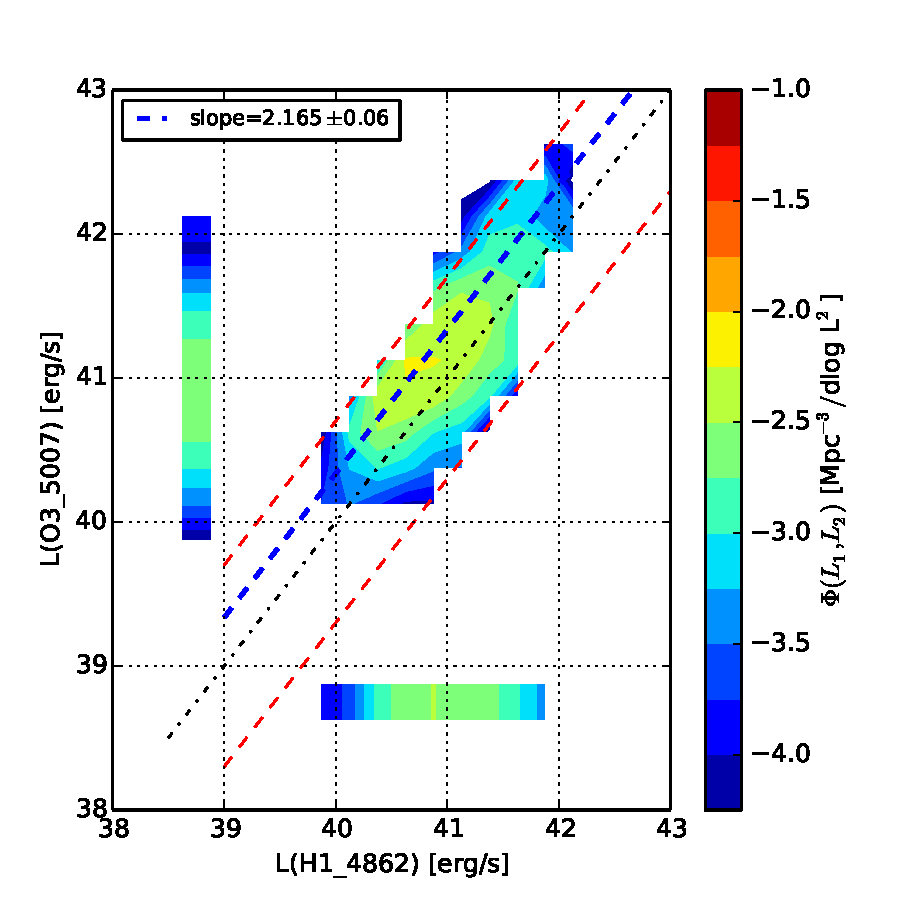
\includegraphics[width = 0.5\textwidth]{Plots/cond_lum.pdf}
 \label{fig:cond-lum}
  \caption{The conditional luminosity function between H$\beta$ and [O III] using the same galaxies as in Figure~\ref{fig:line-ratios}.  The black and red lines are the conditional luminosity function (and 1 sigma) from DEEP2 survey).
 }
 \end{figure}

 We start with dark matter simulations generated by Stanford group (led by Risa
Wechsler, which is part of WFIRST Simulation WG and belongs to the EXPO SIT)
that contain galaxies up to 5-sigma detection limit of grizY = [27.5, 27.0,
26.4, 25.9, 24.0] over 10313 sq. degrees.  Each of the galaxy contain its own
spectral energy distribution which are generated to fit most updated luminosity
function and color evolution measurement. Galaxy magnitudes and shapes are
affected by shear and magnification. We then measured and validated the
correlation function and luminosity function of [O III] selected galaxies (with
WFIRST detection limits) (see Figure~\ref{fig:corr-func}. Next, we plan to apply
the measured line ratios as described in Figure~\ref{fig:line-ratios} to all the
galaxies and reapply the WFIRST detection limits to create a realistic WFIRST
emission line galaxy catalog (with  [O III] as the main galaxy targets), and
assess the effects on BAO peak position due to the possible smearing by
mis-identifying the H$\beta$ as [O III]. In addition to the mocks themselves, it
will be important for us to identify which aspects of the emission lines we
think are close to reality, which are of the right order of magnitude, and which
could be qualitatively different from the real Universe. We envision that we
would continue improving these up to the point where we have the real WFIRST
data.

 In addition, we have also released a code that calculates the interloper
 fraction (Wong, Pullen \& Ho): a Python-based program that applies secondary
 line identification and photometric cuts to mock galaxy surveys, in order to
 simulate interloper identification. We also have a module specifically designed
 to do WFIRST and predict interloper rates for WFIRST \citep{Wong:2016eku}.

 \begin{figure}
 %\includegraphics[width = 3.5in]{corr-func.pdf}
 \label{fig:corr-func}
 \caption{The correlation function of [O III] galaxies with WFIRST detection limit within our 10,000 sq.deg simulations.
 }
 \end{figure}

\subsubsection{H$\alpha$ emitter number density forecasts.} %Simulating Realistic Emission Line Galaxies}

%Wang and Merson have focussed so far on investigating the emission line
%properties of galaxies as predicted by the open-source semi-analytical galaxy
%formation model, \textsc{Galacticus} \citep{Benson:2010kx,Benson2012}). The %first stage of
%this work has been to examine the H$\alpha$ number counts predicted by the model
%and compare the predicted cumulative number density of H$\alpha$ emitters to
%observations from the WISP survey \citep{Colbert:2013ita,Mehta:2015}. By
%adjusting the strength of dust attenuation we are able to obtain %\textsc{Galacticus}
%counts that are in agreement with the WISP observations. I have therefore used
%\textsc{Galacticus} to make predictions for the number density of H$\alpha$ %emitters that will be detected for WFIRST.  Assuming a flux limit of $10^{-16}$ %erg/s/cm$^2$,
%\textsc{Galacticus} predicts WFIRST to observe a number density of 26,000-29,000
%H$\alpha$ emitters per square degree over the redshift range 0.5 $\leq$ z $\leq$
%2. I am now finalizing a paper discussing this work. In addition they have also
%been working on extracting equivalent widths and SEDs for \textsc{Galacticus} %galaxies.
%Code to extract these properties has been included in \textsc{Galacticus}, though these
%features are still be be tested.

% Other WFIRST progress that are not yet a deliverable:
% - We are working on constraining the intrinsic alignment models using filaments constructed from spectroscopic surveys. The idea being that in WFIRST, we can do this for the first time using photometric survey and spectroscopic survey together and mitigating the strongest astrophysical systematic -- intrinsic alignment by modeling it out.  We have measured the intrinsic alignments with LOWZ galaxies and the paper is in prep right now. (Chen, Ho, Mandelbaum, Blazek et al.)

In work led by Merson, Wang, Benson, Kiessling and Rhodes the open source
semi-analytical galaxy formation model, \textsc{Galacticus}
\citep{Benson2010kx,Benson2012}, was used to predict the H${\rm \alpha}$-emitter number counts and redshift distributions for the
WFIRST GRS. This work is published in \citet{Merson2017}.

A four square degree lightcone catalogue was constructed by processing
the dark matter merger trees of the Millennium Simulation
\cite{Springel05} with the \textsc{Galacticus} model. Emission lines
are modelled in \textsc{Galacticus} by interpolating over a library of
emission line luminosities obtained from the \textsc{Cloudy}
\cite{Ferland13} code and stored as a function of hydrogen (HI),
helium (HeI) and and oxygen (OII) ionising luminosities, as well as
the hydrogen gas density and metallicity of the interstellar medium
(ISM). The emission line luminosities are then processed to
incorporate attenuation due to interstellar dust, which can be
modelled using several different methods. Merson and collaborators
consider three dust methods from \citet{Ferrara99}, \citet{Charlot00} and \citet{Calzetti00}. However, it is worth noting that any user-specified dust method can be used in conjunction with \textsc{Galacticus}.

\begin{figure}
  \centering
  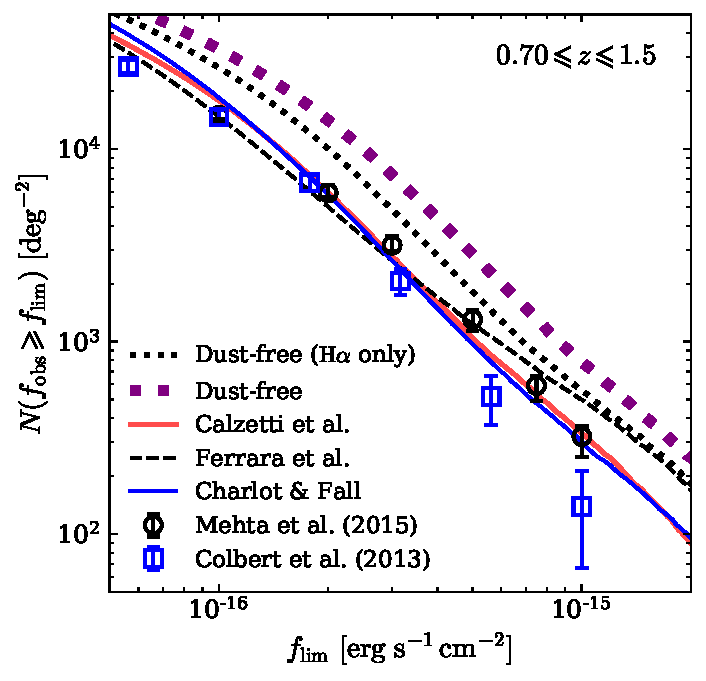
\includegraphics[width=3.5in]{Plots/merson17LightconeHalphaCumulativeCounts.pdf}
  \caption{Predictions for the cumulative H${\rm \alpha}$ flux counts
    for the redshift range $0.7<z<1.5$ from a \textsc{Galacticus}
    lightcone mock catalogue. The various lines show the predictions
    for the pure H${\rm \alpha}$ fluxes and the H${\rm \alpha}$ fluxes
    when blended with NII (H${\rm \alpha}+{\rm NII}$), assuming either
    no dust attenuation or attenuation using one of three methods:
    Ferrara \textit{et al.} (1999) \protect\cite{Ferrara99}, Charlot
    \& Fall (2000) \protect\cite{Charlot00} or Calzetti \textit{et al.} (2000) \protect\cite{Calzetti00}. To be consistent with
    the observed counts from WISP \protect\cite{Colbert13,Mehta2015},
    which are shown by the data points, contamination from NII is
    assumed to contribute 29 per cent to the galaxy luminosity. For
    the Calzetti \textit{et al.} \protect\cite{Calzetti00} method we
    adopt $\tau_{\rm V}\simeq0.83$. For the Charlot \& Fall
    \protect\cite{Charlot00} method we adopt $\hat{\tau}^{\rm ISM}_{\rm V}=0.05$ and $\hat{\tau}^{\rm MC}_{\rm V}=0.04$. When
    applying attenuation due to molecular clouds (MCs) to the Ferrara
    \textit{et al.}  \protect\cite{Ferrara99} method we also assume
    $\hat{\tau}^{\rm MC}_{\rm V}=0.04$.}
  \label{fig:halpha_flux_counts}
\end{figure}

First, the \textsc{Galacticus} predictions for the cumulative counts of H${\rm
\alpha}$-emitting galaxies over the redshift range $0.7\leqslant z\leqslant 1.5$
obtained with each dust method are compared with the latest WISP counts from
\citet{Mehta2015}. The H${\rm \alpha}$ luminosities from \textsc{Galacticus} are
corrected to introduce contamination due to NII by assuming that NII contributes
29 per cent to the observed emission line luminosity. A fixed NII contamination
was chosen to be consistent with the WISP analyses of \citet{Colbert13} and
\citet{Mehta2015}. By adjusting the parameters used by two of these dust models,
the \citet{Charlot00} method and the \citet{Calzetti00} dust law, the authors
are able to obtain predicted cumulative H${\rm \alpha}$ flux counts from
\textsc{Galacticus} that are consistent with the observed counts of \citet{Mehta2015} down to a flux limit of $1\times 10^{-16}{\rm
erg}\,{\rm s}^{-1}{\rm cm}^{-2}$ (see Figure~\ref{fig:halpha_flux_counts}).
Adopting the Ferrara \textit{et al.} \citet{Ferrara99} dust method yields counts
that agree with the observations for flux limits fainter than approximately
$5\times 10^{-16}{\rm erg}\,{\rm s}^{-1}{\rm cm}^{-2}$, but yield an excess in
the number counts for the brightest fluxes. Overall the authors find that down
the expected flux limits of the WFIRST mission, the \textsc{Galacticus} model is
able to predict number densities that are consistent with existing observations
from the WISP survey. Although the lightcone used in this analysis has a small
area on the sky, it is expected that cosmic variance has little effect on the
predicted number counts. Since the lightcone analysis is time-consuming and
expensive in computing resources, the lightcone used in this study was limited
in size to 4 sq deg, in order to provide timely input to WFIRST. However, the
authors plan to build significantly larger lightcones in future work.

After setting the strength of the dust attenuation for each method the
authors then examine whether these chosen attenuation strengths yield
reasonable matches to the observational estimates for the distribution
of optical depth (at the observer-frame H${\rm \alpha}$ wavelength)
and the H${\rm \alpha}$ line luminosity function. For each of the dust
models, \textsc{Galacticus} predicts optical depths that are
consistent within error with the optical depth estimates from WISP
\citep{Dominguez13}, though the \textsc{Galacticus} optical depths do
not show any increase with observed H${\rm \alpha}$ luminosity, as has
been suggested in the literature. The predicted luminosity function
from \textsc{Galacticus} is consistent with the H${\rm \alpha}$
luminosity function from WISP as measured by \citet{Colbert13} over the redshift range $0.9\leqslant z \leqslant 1.5$. Comparison with the luminosity functions from HiZELS \citep{Sobral13} at $z\simeq 0.84$, $z\simeq 1.47$ and $z\simeq 2.23$
shows that with these chosen dust attenuations \textsc{Galacticus} is
able to reproduce the $z\simeq 0.84$ luminosity function, but becomes
progressively a worse fit towards higher redshift, especially at
$z>2$. This suggests that the dust methods may be lacking some
redshift evolution or dependence on other galaxy properties, or that
the \textsc{Galacticus} emission line luminosities are the
incorrect\ strength. Investigating these possibilities requires
rigorous calibration of the \textsc{Galacticus} model, which will be
carried out in future work.

\begin{table*}
\centering
\caption{Predicted cumulative number of H${\rm \alpha}$-emitting
  galaxies per square degree for the WFIRST GRS, assuming a redshift
  range of $0.5\leqslant z\leqslant 2$. The upper half of the table
  shows the counts for NII contaminated fluxes, whilst the lower half
  of the table shows the counts when NII contamination is
  removed. Predicted counts are reported for three dust methods:
  \citet{Calzetti00}, \citet{Charlot00} and \citet{Ferrara99}. For the Ferrara \textit{et al.} method we include attenuation due to molecular clouds (MCs). The
  strength of the attenuation for the various methods are the same as
  in Fig.~\ref{fig:halpha_flux_counts}. Note that the flux limits
  assume contamination by NII, which is set at 29 per cent of the
  total flux, as adopted by \citet{Colbert13}. The efficiency of each survey is
  instrumentation dependent, and has not been included.}
\begin{tabular}{|c|c|c|c|}
\hline
Flux limit&\multicolumn{3}{|c|}{Dust method used with \textsc{Galacticus}}\\
${\rm erg}\,{\rm s}^{-1}{\rm cm}^{-2}$&Calzetti \textit{et al.} (2000) & Charlot \& Fall (2000) & Ferrara \textit{et al.} (1999, inc. MCs)\\
\hline\hline
\multicolumn{4}{|c|}{\textsc{Cumulative counts including NII contamination}}\\
$1\times 10^{-16}$&26344&28958&26730\\
$2\times 10^{-16}$&9169&10439&10571\\
$3\times 10^{-16}$&4675&5378&6013\\
\hline
\multicolumn{4}{|c|}{\textsc{Cumulative counts with NII removed}}\\
$1\times 10^{-16}$&15833&17660&16938\\
$2\times 10^{-16}$&5202&5971&6557\\
$3\times 10^{-16}$&2628&2978&3751\\
\hline
\end{tabular}
\label{tab:cumulativeFluxCounts}
\end{table*}

Finally, the \textsc{Galacticus} lightcone is used to present predictions for
the redshift distribution and the differential and cumulative H${\rm \alpha}$
flux counts for the WFIRST GRS, as well as two surveys mimicking a Euclid-like
selection. These predicted cumulative flux counts to are compared to forecasts
from \citet{Mehta2015} and empirical models originally presented by
\citet{Pozzetti15}. The \textsc{Galacticus} forecasts have counts that are
consistent with those of \citet{Pozzetti15} and about 30 per cent lower than
those of \citet{Mehta2015}. The deficit compared to the Mehta \textit{et al.}
forecasts could be due to Mehta \textit{et al.} using the OIII line to
extrapolate the number of H${\rm \alpha}$ emitters for $z\gtrsim1.6$. For a
WFIRST GRS with redshift range $0.5\leqslant z\leqslant 2$ and flux limit of
$1\times 10^{-16}{\rm erg}\,{\rm s}^{-1}{\rm cm}^{-2}$ \textsc{Galacticus}
predicts a number density between 26,300 and 29,000 galaxies per square degree,
prior to removal of NII contamination, and 29 per cent lower with NII removed.
Note that all the H${\rm \alpha}$-emitter counts discussed in this paper are
expected number counts of target galaxies for spectroscopy, and \emph{not} the
counts of galaxies with redshift measurements. The latter will depend on the
redshift purity and completeness for each survey, which in turn depends on
instrumentation and noise parameters.

\begin{summary}
In this section, we have illustrated that our multiple simulation efforts
complement each other in different ways. LogNormal and Fast simulations with
both positions and shapes,  are useful for pipeline testing and constructing
covariance matrices. The more realistic simulations will test various assumption
and requirements we make for WFIRST HLS. For example, do we need higher
resolution in the grism to disentangle the [O III] and  H$\beta$? Do any of
these line ratios or galaxy properties depend on environment?  Would it lead to an environment dependent BAO smearing if we do not take these into account?  As
we develop more realistic galaxy simulations such as those with \textsc{Galacticus}, we will be able to use the appropriate prescription for
galaxy properties we cannot measure with current observations and make our final
WFIRST simulation as realistic and physically driven as possible. We will examine a variety of other properties of emission line galaxies, including the distribution of OIII luminosities fluxes and the contamination from NII.
This will allow us to have the best tool to develop both the methods for modeling and interpretation of cosmological measurements from WFIRST, and release the most
realistic WFIRST galaxy catalog to the public before WFIRST launch.
\end{summary}

\subsection{Improving our Knowledge of the H$\alpha$ Luminosity Function}

\begin{summaryii}
Knowing the H$\alpha$ and [OIII] luminosity functions is critical in order to optimize the WFIRST GRS. We are addressing current limitations in our knowledge using a newly available set of HST spectroscopic data within the WISP collaboration.
\end{summaryii}

In order to trace the galaxy distribution through z$\sim$2.7, the future WFIRST
surveys will make use of H$\alpha$ and [OIII] selected emission line galaxies.
These two lines will allow WFIRST to cover the redshift range 1$<$z$<$2
(H$\alpha$) and 2$<$z$<$2.7 ([OIII]) respectively. Therefore, knowing the
expected number of H$\alpha$ galaxies in the survey volume is required and the
study of the H$\alpha$ luminosity function (LF) become fundamental in order to
optimize the planned redshift surveys. However, despite the numerous works on
this topic, given the high uncertainties associated to the H$\alpha$ LF
determination, a sufficiently precise measure is still lacking
(Figure~\ref{fig:img_depths}). Additionally, the samples of emission-line
galaxy are expected to be affected by a complex selection function that depends
on galaxy luminosity, size, line equivalent width and also on contamination from
mis-identified single emission-line galaxies at different depths.

A newly available set of HST spectroscopic data, gathered in the context of the
WFC3 Infrared Spectroscopic Parallel (WISP) survey \citep{Atek:2010},
of which team members Teplitz and Baronchelli are members, has recently become
publicly available. Currently, this survey covers a total area of more than
$\simeq$ 2000 sq. arcmin., with thousands of emission lines from a total
of $\sim$500 randomly distributed HST pointings identified between z=0.3 and
z=1.5. Thousands of emission lines from a total of $\sim$500 randomly
distributed HST pointings have already been identified by the WISP team, between z=0.3 and z=1.5. The spectroscopic capabilities of HST+WFC3 are comparable to those that WFIRST can reach over a 2-order of magnitude wider area. This fact makes the WISP survey a particularly suitable test bench to optimize the future WFIRST surveys.

The accurate constraint of the parameters defining the line LF ($\phi^{*}*, L^{*}, \alpha$) is hindered by their high correlation. Therefore, estimating these parameters requires uniform sampling of both the bright and faint ends of the luminosity distribution. In the next months, in the context of a collaboration involving both WISP and SIT members, Teplitz, Baronchelli and Wang, are planning to obtain the most accurate estimate, to-date, of the H$\alpha$ and [OIII] LFs in the redshift range 0.7-1.6 and 2-2.2 respectively. This result will be achieved by combining deep and shallow data from various HST-WFC3 slitless spectroscopic surveys: WISP (\citet{Atek:2010}, PI: Malkan, M.), the SN followup of the CANDELS survey (SN-CANDELS, PI: Riess, A.), 3D-HST (\citet{VanDokkum:2011,Brammer:2012}, PI: Van Dokkum) and AGHAST (A Grism H-Alpha SpecTroscopic survey in the GOODS-N, PI: B. Weiner).
%In the next months, by combining deep and shallow WISP, CANDELS SN and 3D-HST+AGHAST datasets, Harry Teplitz, Ivano Baronchelli and Yun Wang, in a collaboration between the SIT and the WISP teams, are planning to obtain the most acurate estimate, to-date, of the H$\alpha$ and [OIII] LFs in the redshift range 0.7-1.6 and 2-2.2 respectively.
Since previous studies suggest a substantial brightening of $L^{*}_{H\alpha}$ (Figure~\ref{fig:img_depths}), this study will be performed by dividing the sample in three redshift bins between z=0.7 and z=1.6. Even if split, the combined sample is large enough to allow for an uniform coverage of the $H\alpha$ luminosity range, from few \% of $L^{*}_{H\alpha}$ to many times $L^{*}_{H\alpha}$.

\begin{figure}[!t]
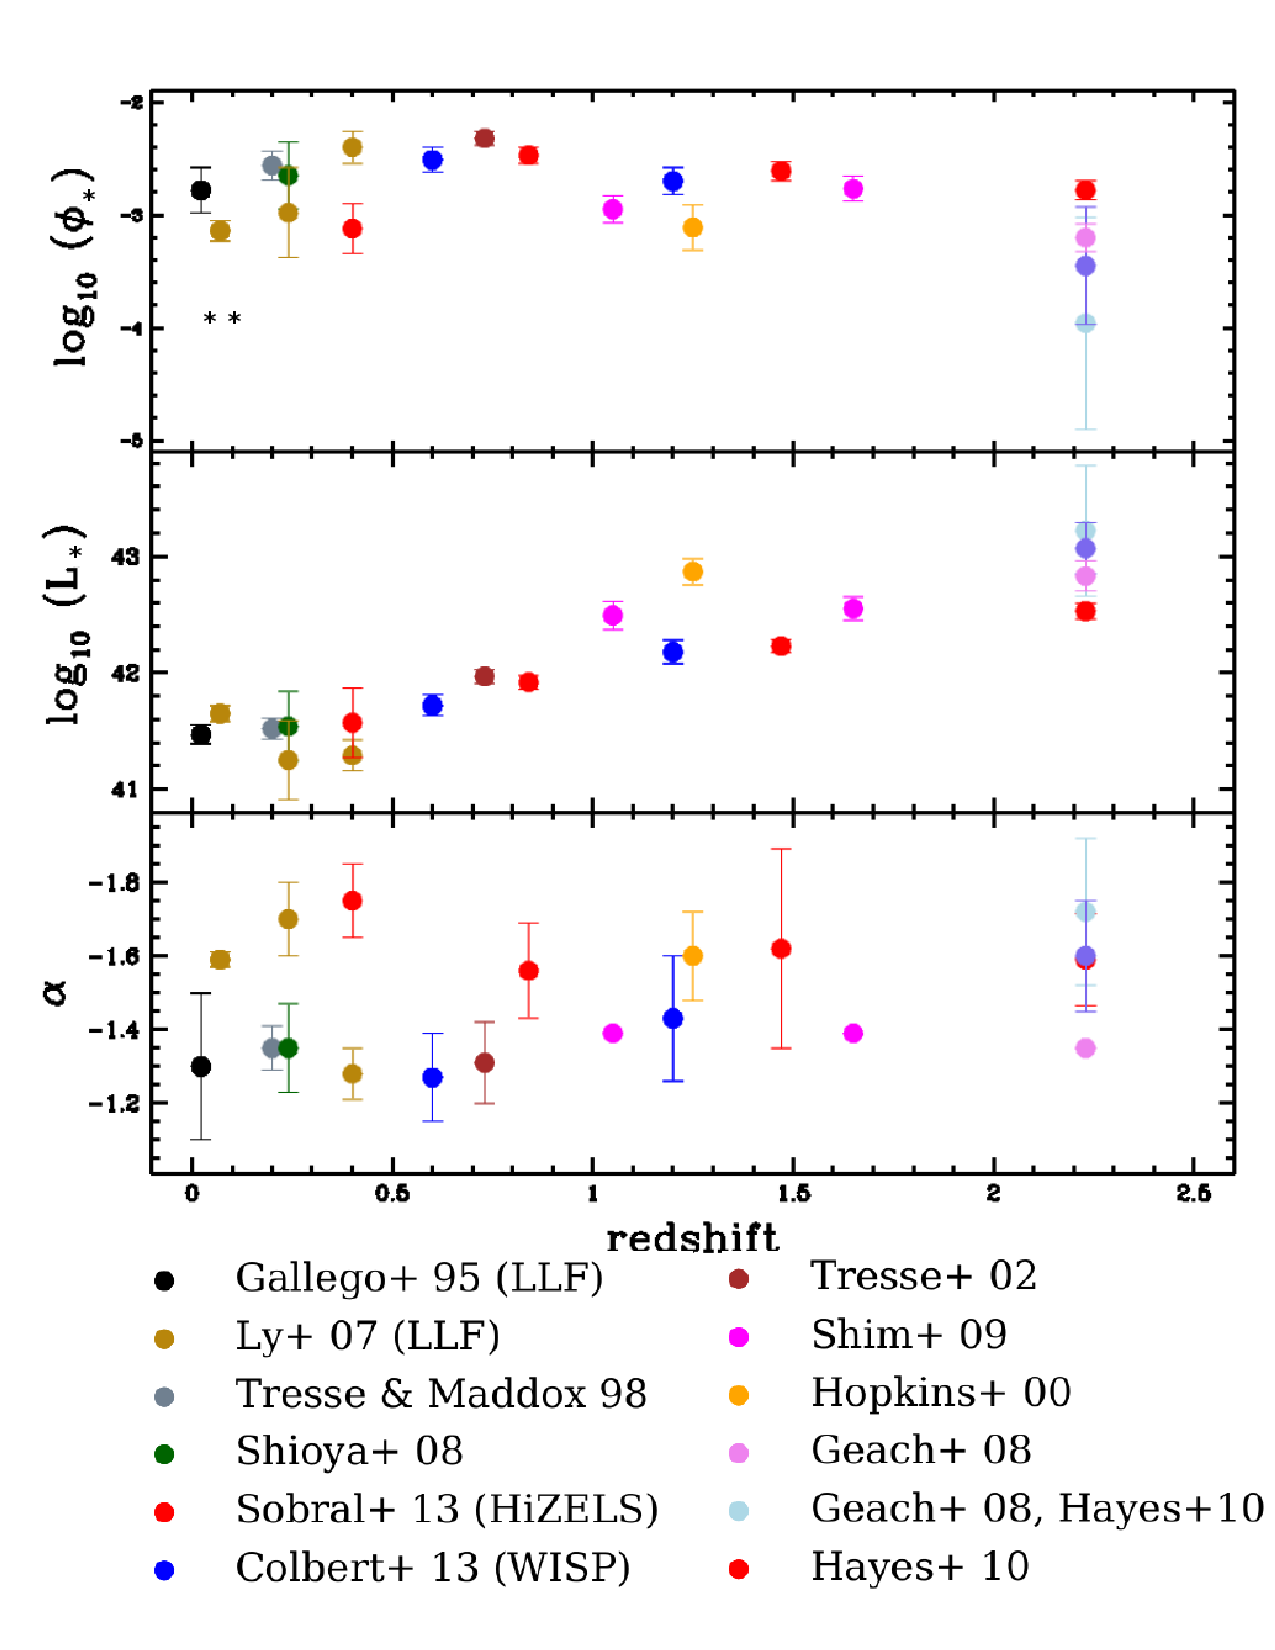
\includegraphics[width=0.5\textwidth]{Plots/HA_LF.pdf}
%\includegraphics[width=7.5cm]{WFIRST_WISP_comparison.eps}
\caption{H$\alpha$ LF as estimated in various surveys. The uncertainties on the different parameters defining the LF are considerable. The aim of this project is to measure the most precise H$\alpha$ and [OIII] luminosity functions to-date, in the redshift range 0.7-1.6 and 2-2.2 respectively.}%{\bf 1B)} Redshift and wavelength coverage for planned WFIRST surveys compared with WISP and Euclid. The shaded regions indicate the full wavelength and redshift ranges of
\label{fig:img_depths}
\end{figure}

Above z=1.6, the H$\alpha$ line is redshifted outside the detectable wavelength
range and since single line emitters are considered H$\alpha$ by default, the
ability to confirm the identification of [OIII] lines is limited to bright lines
with clear shapes. Greatly extending the small dataset used in
\citet{Colbert:2013ita}, the newly released WISP data will allow us to better
constrain the contamination of the H$\alpha$ selected sample, and the loss of
completeness of the [OIII] sample. We will use the multi-wavelength dataset on
3D-HST + AGHAST to identify a combination of colors that could possibly mitigate
this problem.

The identification of the spectral lines and the measure of their fluxes is
fundamental for all the successive part of the LF project here described, but it
can not be completely performed by an automatic algorithm. Thanks to the same
collaboration involving both the SIT and WISP team members, automatic softwares
have already been optimized to i) remove low S/N detections and some of the
contaminating false detections and ii) measure the total line fluxes after their
identification. However, the human interaction is required to visually identify
each detected line (mostly H$\alpha$ and [OIII], but also OII, H$\beta$ and
SII), to perform high quality continuum and line fits, and to remove not
automatically identified contaminants. In the past weeks, the work has been
focused on these tasks. As a result, a large dataset of thousands of objects
with measured line fluxes and corresponding redshift is now available.
% Using the same data, the continuum luminosity, galaxy size and EW distribution functions for line emitters can be constrained.

At the end of the work described in this section, for which more than a semester is still reasonably required, the results will bring to a publication, in one of the major journals, with the co-authorship of Teplitz, Baronchelli and Wang.


 \subsection{Cosmological Forecasting and Data Analysis Algorithms}

 \begin{summaryii}
  We have developed software package to make quick forecasts on basic dark energy parameters from higher order statistics, incluging power spectrum and bispectrum multipoles. This light and agile software package will be the backbone of our GRS proto-pipeline effort.
  \end{summaryii}

 The key dark energy constraints from the WFIRST GRS will result from the BAO and
 RSD measurements from the two-point statistics of the observed galaxy field.
 Similar measurements from the higher order statistics are weaker and currently
 are considered less robust. Cosmological constraints from higher order
 statistics scale very steeply with the number density and since WFIRST GRS will
 provide very dense galaxy samples they may significantly enhance the yield from
 the standard two-point BAO/RSD analysis. We also expect the methods of analyzing
 higher order statistics to become more robust and standardized by the time of
 WFIRST launch. Because of these considerations it would be helpful to have a
 higher order statistics forecasting tool. We have developed software package to
 make forecasts on basic dark energy parameters from higher order statistics.
 The main assumptions are similar to the ones made in the standard
 power-spectrum forecasting tool used for baseline WFIRST predictions. We will
 work on integrating this software with the standard forecasting tool developed
 by our SIT. While the key design decisions will still be based on the
 two-point statistics forecasts, knowing how different choices will effect higher
 order analysis will be very informative.

 The KSU group has assembled a fast and lightweight set of tools for analyzing
 the WFIRST GRS data. Currently this toolset starts from the redshift catalogue
 and the visibility cube and produces the measurements of power spectrum
 multipoles. The multipoles are then analyzed to extract the BAO and RSD signal
 from them. The BAO extraction algorithms replicate the analysis of the final
 BOSS DR12 sample. The RSD analysis is currently simplistic and uses the linear
 model. We will update this toolset by implementing more realistic RSD models.
 The toolset will eventually be linked to the redshift catalogue and visibility
 cube producing software. This software will provide the backbone of our BAO/RSD
 proto-pipeline and will be validated with high fidelity WFIRST simulations.


 \begin{summary}[Future Work on Galaxy Redshift Survey]
 \begin{enumerate}
 \item We will keep refining and solidifying the scientific requirements;
 \item We will pursue our light-cone simulations and release mock catalogs to the community when publishing our results;
 \item We will pursue our effort with image simulation, relying on the light-cone simulation to incorporate realistic galaxy distributions and properties;
 \item We will continue our pseudo-pipeline effort;
 \item \Oli{TO BE CONTINUED}.
 \end{enumerate}
 \end{summary}
